\chapter{\IfLanguageName{dutch}{Stand van zaken}{State of the art}}%
\label{ch:stand-van-zaken}

% Tip: Begin elk hoofdstuk met een paragraaf inleiding die beschrijft hoe
% dit hoofdstuk past binnen het geheel van de bachelorproef. Geef in het
% bijzonder aan wat de link is met het vorige en volgende hoofdstuk.

% Pas na deze inleidende paragraaf komt de eerste sectiehoofding.
\section{Focus op Authenticatie en Beveiliging}\\

De ontwikkeling van mobiele applicaties heeft de afgelopen jaren aanzienlijke vooruitgangen geboekt, waarbij beveiliging en de keuze van het platform cruciale factoren zijn geworden. Gezien de steeds grotere hoeveelheid persoonlijke gegevens die mobiele applicaties verwerken, is de noodzaak voor robuuste beveiligingsmaatregelen urgenter dan ooit. De trends in mobiele applicaties die steeds meer persoonlijke gegevens verwerken, benadrukken het belang van een sterke beveiliging \autocite{build382022}. Dit onderzoek richt zich op de ontwikkeling van een mobiele applicatie met .NET MAUI, met speciale aandacht voor authenticatie en beveiliging. Een essentieel aspect van dit proces is de implementatie van JSON Web Tokens (JWT), het veilig hashen van wachtwoorden en het creëren van een betrouwbare loginpagina. Deze technieken worden ingezet om zowel de veiligheid als de efficiëntie van de gebruikerservaring te waarborgen en zijn van vitaal belang voor de bescherming van gevoelige gegevens tegen ongeautoriseerde toegang. De implementatie van technieken zoals JWT en wachtwoordhashing zijn best practices die worden aanbevolen in de recente literatuur over mobiele app-beveiliging \autocite{AndrewMakarov}. Daarnaast is het waarborgen van de privacy van gebruikersgegevens in mobiele apps een aanzienlijke uitdaging, zoals beschreven in recente literatuur over de privacy-uitdagingen van mobiele applicaties \autocite{Cybersecurity2018}. Deze methoden reflecteren de recente trends in mobiele app-beveiliging, best practices voor mobiele app-ontwikkeling en de uitdagingen van dataprivacy in mobiele applicaties. \\

.NET MAUI (Multi-platform App UI) is gekozen als ontwikkelplatform vanwege de mogelijkheid om een enkele codebase te gebruiken voor zowel Android als iOS. Dit vereenvoudigt de ontwikkeling, onderhoud en distributie van de applicatie. .NET MAUI bouwt voort op Xamarin, maar biedt betere prestaties, een verbeterde gebruikersinterface en diepere integratie met .NET 7/8 \autocite{Klesman2023}. Deze integratie zorgt voor een robuuste backend die goed samenwerkt met andere .NET-technologieën, zoals ASP.NET Core voor server-side processen en Azure voor cloudgebaseerde diensten. Dit maakt het platform bijzonder aantrekkelijk voor ontwikkelaars die reeds ervaring hebben met C# en het .NET-ecosysteem, aangezien het hen in staat stelt om efficiënter te werken en gebruik te maken van hun bestaande kennis. Verder, wanneer we de vergelijking maken met andere frameworks zoals React Native en Flutter, blijkt .NET MAUI te bieden wat betreft prestaties en platformintegratie een sterke keuze te zijn voor cross-platform ontwikkeling \autocite{Kuppan2024}. \\

Een belangrijk aspect van de beveiliging in mobiele applicaties is de implementatie van JSON Web Tokens (JWT) voor authenticatie. JWT wordt steeds vaker gekozen boven traditionele sessiebeheermechanismen vanwege de efficiëntie en schaalbaarheid. In tegenstelling tot traditionele sessiebeheermechanismen, waarbij gegevens op de server worden opgeslagen, bevat een JWT-token zelf de versleutelde gebruikersinformatie. Dit maakt snellere verificatie mogelijk, omdat de server geen sessie-informatie hoeft op te slaan of te raadplegen voor elke gebruikersaanroep.
Het gebruik van JWT biedt een veilige manier om gebruikers te verifiëren zonder afhankelijk te zijn van server-side sessies. Dit vermindert de belasting van de server en maakt de applicatie schaalbaarder, wat vooral voordelig is voor applicaties met veel gelijktijdige gebruikers, zoals sociale netwerken en online marktplaatsen. Daarnaast draagt JWT bij aan het verbeteren van de beveiliging door het minimaliseren van de kans op sessie-gestuurde aanvallen, zoals cross-site scripting (XSS) en cross-site request forgery (CSRF).
De beveiliging van JWT-tokens is echter cruciaal, aangezien een gelekt token kan leiden tot ongeautoriseerde toegang. Om dit te voorkomen, worden tokens alleen via HTTPS verzonden en voorzien van een beperkte geldigheidsduur. Dit maakt het moeilijker voor aanvallers om een gestolen token langdurig te misbruiken. Het implementeren van JWT voor authenticatie wordt dan ook breed aanbevolen in de literatuur over mobiele app-beveiliging \autocite{Gao2023}. \\

\begin{figure}
    \centering
    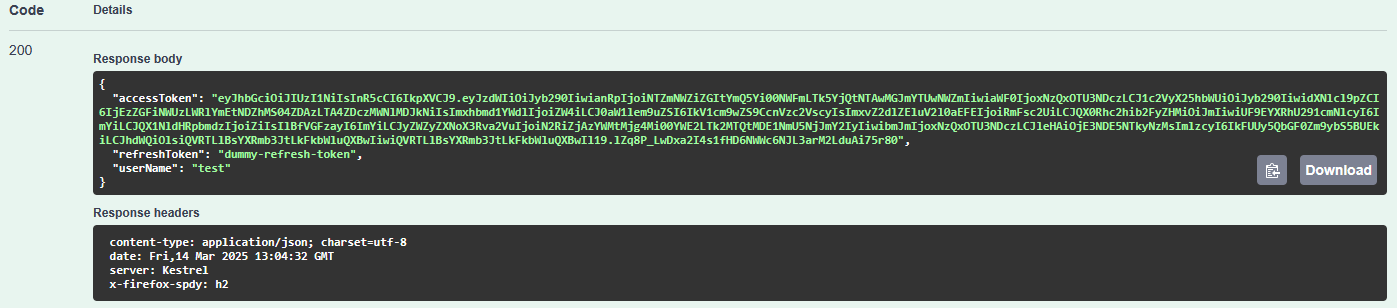
\includegraphics[width=0.8\textwidth]{token.png}
    \caption[Token]{Het resultaat van een succesvolle login met een gegenereerde token als resultaat.}
\end{figure}

Om wachtwoorden veilig op te slaan, worden cryptografische hashing-algoritmes zoals bcrypt en PBKDF2 gebruikt, omdat deze bestand zijn tegen brute-force aanvallen \autocite{Gupta2022}. Bij een brute-force aanval proberen hackers systematisch verschillende wachtwoordcombinaties te raden, maar door sterke hashing-algoritmes toe te passen, kan dit proces aanzienlijk worden vertraagd.
Daarnaast wordt salting toegepast, waarbij een willekeurige waarde aan het wachtwoord wordt toegevoegd voordat het wordt gehasht. Dit maakt het moeilijker voor aanvallers om vooraf gegenereerde lijsten met veelgebruikte wachtwoorden en combinaties, zoals die in dictionary-aanvallen, effectief te gebruiken \autocite{Arias2025}.
Deze maatregelen zijn essentieel, aangezien onderzoek aantoont dat zwakke hashing-algoritmes, zoals MD5 en SHA1, een veelvoorkomende kwetsbaarheid vormen in mobiele applicaties. Hackers maken vaak misbruik van verouderde encryptiemethoden om toegang te krijgen tot gevoelige gegevens \autocite{ReesCarter2024}. \\

De loginpagina is een cruciaal onderdeel van de applicatie en vereist een balans tussen gebruiksvriendelijkheid en beveiliging. Het is essentieel dat gebruikers eenvoudig toegang krijgen tot hun account zonder dat dit ten koste gaat van de veiligheid. Gebruikers kunnen zich aanmelden met hun e-mailadres en wachtwoord, waarna validatie plaatsvindt via een backend die JWT-tokens genereert en verstuurt.
Om aanvallen zoals credential stuffing te voorkomen waarbij geautomatiseerde systemen proberen in te loggen met gestolen inloggegevens, wordt een limiet ingesteld op het aantal mislukte inlogpogingen. Dit voorkomt dat aanvallers massaal inlogpogingen uitvoeren en zo het systeem proberen te misbruiken \autocite{Chinnasamy2025}.
Daarnaast worden aanvullende beveiligingsmaatregelen overwogen, zoals tweefactorauthenticatie (2FA) via Azure AD of Google. Deze technologieën voegen een extra beveiligingslaag toe, doordat gebruikers niet alleen een wachtwoord, maar ook een tijdelijke code moeten invoeren die wordt gegenereerd door een app of via SMS wordt verzonden \autocite{Jurisons2024}.

\begin{figure}
    \centering
    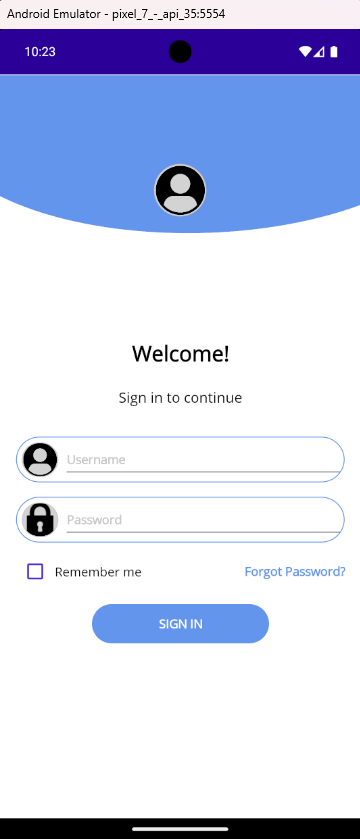
\includegraphics[width=0.8\textwidth]{login.png}
    \caption[Token]{Het inlogscherm die ik heb gemaakt voor ATS.}
\end{figure}

\begin{listing}
  \begin{minted}{python}
    import pandas as pd
    import seaborn as sns

    penguins = sns.load_dataset('penguins')
    sns.relplot(data=penguins, x="flipper_length_mm", y="bill_length_mm", hue="species")
  \end{minted}
  \caption[Voorbeeld codefragment]{Voorbeeld van het invoegen van een codefragment.}
\end{listing}


\begin{table}
  \centering
  \begin{tabular}{lcr}
    \toprule
    \textbf{Kolom 1} & \textbf{Kolom 2} & \textbf{Kolom 3} \\
    $\alpha$         & $\beta$          & $\gamma$         \\
    \midrule
    A                & 10.230           & a                \\
    B                & 45.678           & b                \\
    C                & 99.987           & c                \\
    \bottomrule
  \end{tabular}
  \caption[Voorbeeld tabel]{\label{tab:example}Voorbeeld van een tabel.}
\end{table}

